We will have time to learn about each of the performance analysis tools in more detail in the rest of this chapter, but in this section, we will do a quick end-to-end example and analyze the performance of a simple program. This will show you what the typical performance analysis flow looks like and how different tools are used.

There is also a hidden agenda: by the end of this section, you will come to believe that you should never guess about performance.

Any real-world program that you may have to analyze and optimize is likely to be large enough to take many pages in this book, so we will use a simplified example. This program sorts substrings in a very long string: suppose we have a string S, such as "abcdcba" (this is not so long; our actual strings will have millions of characters). We can have a substring starting from any character in this string, for example, the substring S0 starts with the offset 0 and, therefore, has the value "abcdcba". The substring S2 starts with offset 2 and has the value "cdcba", and the substring S5 has the value "ba". If we were to sort these substrings in decreasing order using the regular string comparison, the order of the substrings would be S2, then S5, then S0 (in order of the first characters, 'c', 'b', and 'a', respectively).

We can use the STL sort algorithm, std::sort, to sort the substrings if we represent them with a character pointer: swapping two substrings now involves just swapping the pointers while the underlying string remains unchanged. Here is our example program:

\hspace*{\fill} \\ %插入空行
\noindent
\textbf{01\_substring\_sort.C}
\begin{lstlisting}[style=styleCXX]
bool compare(const char* s1, const char* s2, unsigned int l);
int main() {
	constexpr unsigned int L = …, N = …;
	unique_ptr<char[]> s(new char[L]);
	vector<const char*> vs(N);
	  … prepare the string …
	size_t count = 0;
	system_clock::time_point t1 = system_clock::now();
	std::sort(vs.begin(), vs.end(),
	  [&](const char* a, const char* b) {
		++count;
		return compare(a, b, L);
	});
	system_clock::time_point t2 = system_clock::now();
	cout << "Sort time: " <<
	  duration_cast<milliseconds>(t2 - t1).count() <<
	  "ms (" << count << " comparisons)" << endl;
}
\end{lstlisting}

Note that, in order for this example to compile, we need to include the appropriate header files and write the using declarations for the names we shorten:

\begin{lstlisting}[style=styleCXX]
#include <algorithm>
#include <chrono>
#include <cstdlib>
#include <cstring>
#include <iostream>
#include <memory>
#include <random>
#include <vector>
using std::chrono::duration_cast;
using std::chrono::milliseconds;
using std::chrono::system_clock;
using std::cout;
using std::endl;
using std::minstd_rand;
using std::unique_ptr;
using std::vector;
\end{lstlisting}

In the subsequent examples, we will omit the common header files and the using declarations for common names such as cout or vector.

The example defines a string that is used as the underlying data for the substrings to be sorted and for the vector of substrings (character pointers), but we have not yet shown how the data itself is created. Then, the substrings are sorted using std::sort with a custom comparison function: a lambda expression that calls the comparison function itself, compare(). We use the lambda expression to adapt the interface of the compare() function, which takes two pointers and the maximum string length, to the interface expected by std::sort (just two pointers). This is known as the Adapter Pattern.

In our case, the lambda expression has the second role: in addition to calling the comparison function, it also counts the number of comparison calls. Since we are interested in the performance of the sort, this information may be useful if we want to compare different sorting algorithms (we are not going to do this now, but this is a technique you may find useful in your own performance optimization efforts).

The comparison function itself is only declared in this example, but not defined. Its definition is in a separate file and reads as follows:


\hspace*{\fill} \\ %插入空行
\noindent
\textbf{01\_substring\_sort\_a.C}
\begin{lstlisting}[style=styleCXX]
bool compare(const char* s1, const char* s2, unsigned int l) {
	if (s1 == s2) return false;
	for (unsigned int i1 = 0, i2 = 0; i1 < l; ++i1, ++i2) {
		if (s1[i1] != s2[i2]) return s1[i1] > s2[i2];
	}
	return false;
}
\end{lstlisting}

It is a straightforward comparison of two strings: it returns true if the first string is greater than the second one and false otherwise. We could have just as easily defined the function in the same file as the code itself and avoided the need for the extra file, but even with this small example, we are trying to reproduce the behavior of a real-world program that will likely call many functions scattered across many different files. Therefore, we have the comparison function in its own file, which we call compare.C in  this chapter, and the rest of the example is in one file, example.C.

Lastly, we use the C++ high-resolution timers from the chrono library to measure how long it took to sort the substrings.

The only thing that is missing in our example is the actual data for the string. The substring sort is a fairly common task in many real applications, and each has its own way of acquiring the data. In our artificial example, the data will have to be equally artificial. We can, for example, generate a random string. On the other hand, in many practical applications of substring sort, there is one character that occurs in the string much more often than any other.

We can simulate this type of data as well by filling the string with a single character and then randomly changing a few of them:

\hspace*{\fill} \\ %插入空行
\noindent
\textbf{01\_substring\_sort\_a.C}
\begin{lstlisting}[style=styleCXX]
constexpr unsigned int L = 1 << 18, N = 1 << 14;
unique_ptr<char[]> s(new char[L]);
vector<const char*> vs(N);
minstd_rand rgen;
::memset(s.get(), 'a', N*sizeof(char));
for (unsigned int i = 0; i < L/1024; ++i) {
	s[rgen() % (L - 1)] = 'a' + (rgen() % ('z' - 'a' + 1));
}
s[L-1] = 0;
for (unsigned int i = 0; i < N; ++i) {
	vs[i] = &s[rgen() % (L - 1)];
}
\end{lstlisting}

The size of the string L and the number of substrings N are chosen to have reasonable run times on the machine that was used to run these tests (if you want to repeat the examples, you may have to adjust the numbers up or down depending on the speed of your processor).

Now our example is ready to be compiled and executed:

\hspace*{\fill} \\ %插入空行
\begin{center}
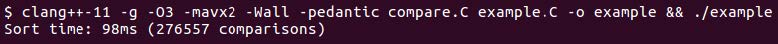
\includegraphics[width=0.9\textwidth]{content/1/chapter2/images/1.jpg}\\
Figure 2.1
\end{center}

The results you will get depend on the compiler you use, the computer you run on, and, of course, on the data corpus.

Now that we have our first performance measurement, the first question you may ask is, how do we optimize it? This is not the first question you should be asking, though. The real first question should be, do we need to optimize? To answer that, you need to have the targets and goals for performance, as well as the data on the relative performance of the other parts of this program; for example, if the actual string is generated from a simulation that takes ten hours, the one hundred seconds it takes to sort it is hardly worth noticing. Of course, we are still dealing with the artificial example, and we won't get very far in this chapter unless we assume that, yes, we have to improve performance.

Now, are we ready to talk about how to optimize it? Again, not so fast: the question now should be, what do we optimize? Or, more generally, where does the program spend the most time? Even in this simple example, it could be the sort itself or the comparison function. We do not have access to the source code of the sort (unless we want to hack the standard library, anyway), but we could insert the timer calls into the comparison function.

Unfortunately, this is unlikely to yield good results: each comparison is pretty fast, timer calls themselves take time, and calling the timer every time the function is called will significantly change the very results we're trying to measure. In a real-world program, such instrumentation with timers is often not practical anyway. You would have to insert timers into hundreds of functions if you didn't know where the time is spent (and how would you know that without any measurements?). This is where the profiler tools come in.

We will learn much more about the profiler tools in the next section. For now, suffice it to say that the following command line will compile and execute the program and collect its runtime profile using the Google profiler from the GperfTools package:

\hspace*{\fill} \\ %插入空行
\begin{center}
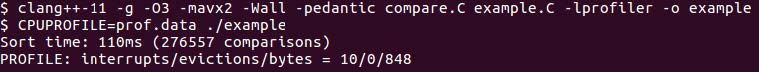
\includegraphics[width=0.9\textwidth]{content/1/chapter2/images/2.jpg}\\
Figure 2.2
\end{center}

The profile data is collected in the file prof.data, as given by the CPUPROFILE environment variable. You may have noticed that the program took longer to run this time. This is an almost unavoidable side effect of performance profiling. We will come back to it in the next section. The relative performance of the different parts of the program should still be correct, assuming the profiler itself is working correctly.

The last line of the output tells us that the profiler has collected some data for us, now we need to display it in a readable format. For the data collected by the Google profiler, the user interface tool is google-pprof (often installed as simply pprof), and the simplest invocation of it just lists every function in the program, along with the fraction of the time spent in that function (the second column):

\hspace*{\fill} \\ %插入空行
\begin{center}
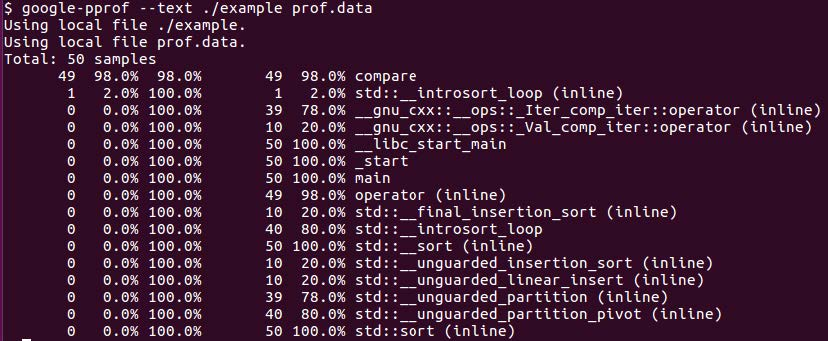
\includegraphics[width=0.9\textwidth]{content/1/chapter2/images/3.jpg}\\
Figure 2.3
\end{center}

The profiler shows that almost all the time is spent in the comparison function compare() and that the sort hardly takes any time at all (the second line is one of the functions called by std::sort and should be considered a part of the time spent in the sort but outside of the comparison). Note that for any practical profiling, we would need more than the 50 samples collected here. The number of samples depends on how long the program runs, and, to get reliable data, you need to accumulate at least a few dozen samples in every function you want to measure. In our case, the result is so glaringly obvious that we can proceed with just the samples we collected.

Since the substring comparison function takes 98\% of the total run time, we have only two ways to improve the performance: we can make this function faster, or we can call it fewer times (many people forget the second possibility and go straight for the first one). The second approach would require the use of a different sort algorithm and is, therefore, outside of the scope of this book. Here we will focus on the first option. Let us again review the code for the comparison function:

\hspace*{\fill} \\ %插入空行
\noindent
\textbf{01\_substring\_sort\_a.C}
\begin{lstlisting}[style=styleCXX]
bool compare(const char* s1, const char* s2, unsigned int l) {
	if (s1 == s2) return false;
	for (unsigned int i1 = 0, i2 = 0; i1 < l; ++i1, ++i2) {
		if (s1[i1] != s2[i2]) return s1[i1] > s2[i2];
	}
	return false;
}
\end{lstlisting}

This is just a few lines of code, and we should be able to understand and predict everything about its behavior. There is the check for comparing a substring to itself, which is definitely faster than actually doing the comparison character by character, so, unless we are sure that the function is never called with identical values for both pointers, this line stays.

Then there is a loop (the body of the loop is comparing the characters one at a time), which we have to do because we do not know which character might be different. The loop itself runs until we find a difference or until we compare the maximum possible number of characters. It is easy to see that the latter condition cannot possibly happen: the string is null-terminated, so, even if all characters in both substrings are the same, sooner or later we will reach the end of the shorter substring, compare the null character at its end with a non-null character in the other substring, and the shorter substring will be considered the lesser of the two.

The only case where we could potentially read past the end of the string is when both substrings start at the same location, but we check for that at the very beginning of the function. This is great: we have found some unnecessary work that we were doing, so we can optimize the code and get rid of one comparison operation per loop iteration. Considering that there aren't many other operations in the loop body, this ought to be significant.

The change in the code is simple enough: we can just remove the comparison (we also do not need to pass the length into the comparison function anymore):

\hspace*{\fill} \\ %插入空行
\noindent
\textbf{03\_substring\_sort\_a.C}
\begin{lstlisting}[style=styleCXX]
bool compare(const char* s1, const char* s2) {
	if (s1 == s2) return false;
	for (unsigned int i1 = 0, i2 = 0;; ++i1, ++i2) {
		if (s1[i1] != s2[i2]) return s1[i1] > s2[i2];
	}
	return false;
}
\end{lstlisting}

Fewer parameters, fewer operations, less code all around. Let's run the program and see how much run time this optimization saved us:

\hspace*{\fill} \\ %插入空行
\begin{center}
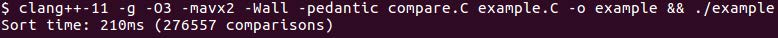
\includegraphics[width=0.9\textwidth]{content/1/chapter2/images/4.jpg}\\
Figure 2.4
\end{center}

To say that this didn't go according to plan would be a major understatement. The original code took 98 milliseconds to solve the same problem (Figure 2.1). The "optimized" code takes 210 milliseconds, despite doing less work (note that not all compilers exhibit this particular performance anomaly on this example, but we're using a real production compiler; there is no trickery here, this could happen to you too).

To wrap up this example, which is actually a much-condensed example from a real-life program, I will tell you that while we were trying to optimize this fragment of code, another programmer was working in a different part of the code and also needed a substring comparison function. When the separately developed pieces of code were put together, only one version of this function was kept, and it happens to be the one we did not write; the other programmer wrote almost the same code:

\hspace*{\fill} \\ %插入空行
\noindent
\textbf{04\_substring\_sort\_a.C}
\begin{lstlisting}[style=styleCXX]
bool compare(const char* s1, const char* s2) {
	if (s1 == s2) return false;
	for (int i1 = 0, i2 = 0;; ++i1, ++i2) {
		if (s1[i1] != s2[i2]) return s1[i1] > s2[i2];
	}
	return false;
}
\end{lstlisting}

Examine this code fragment and the one right before it and see if you can spot the difference.

The only difference is the type of the loop variable: earlier, we used unsigned int, and we were not wrong: the index starts from 0 and advances; we do not expect any negative numbers. The last code fragment uses int, unnecessarily giving up half of the range of the possible index values.

After this code consolidation, we can run our benchmark again, this time with the new comparison function. The result is, again, unexpected:

\hspace*{\fill} \\ %插入空行
\begin{center}
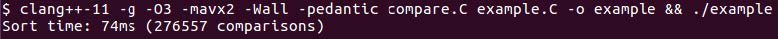
\includegraphics[width=0.9\textwidth]{content/1/chapter2/images/5.jpg}\\
Figure 2.5
\end{center}

The latest version takes 74 milliseconds, faster than our original version (98 milliseconds, Fig 2.1) and much faster than the almost identical second version (210 milliseconds, Fig 2.2).

For the explanation of this particular mystery, you will have to wait until the next chapter. The goal of this section was to convince you to never guess about performance: the "obvious" optimization – doing the exact same computation with less code – backfired spectacularly, and the trivial change that should not have mattered at all – using signed integers instead of unsigned in a function where all values are non-negative anyway – turned out to be an effective optimization.

If the performance results can be so counter-intuitive even in this very simple example, then the only way to make good decisions about performance has to be the measurementdriven approach. In the rest of this chapter, we will see some of the most common tools used to collect performance measurements, learn how to use them, and how to interpret their results.
